\documentclass{article}
\usepackage{graphicx}
\usepackage[margin=1.5cm]{geometry}
\usepackage{amsmath}

\begin{document}

\title{Tuesday Reading Assessment: Chapter 1}
\author{Prof. Jordan C. Hanson}

\maketitle

\section{Properties of Digital Pulses}

\begin{figure}
\centering
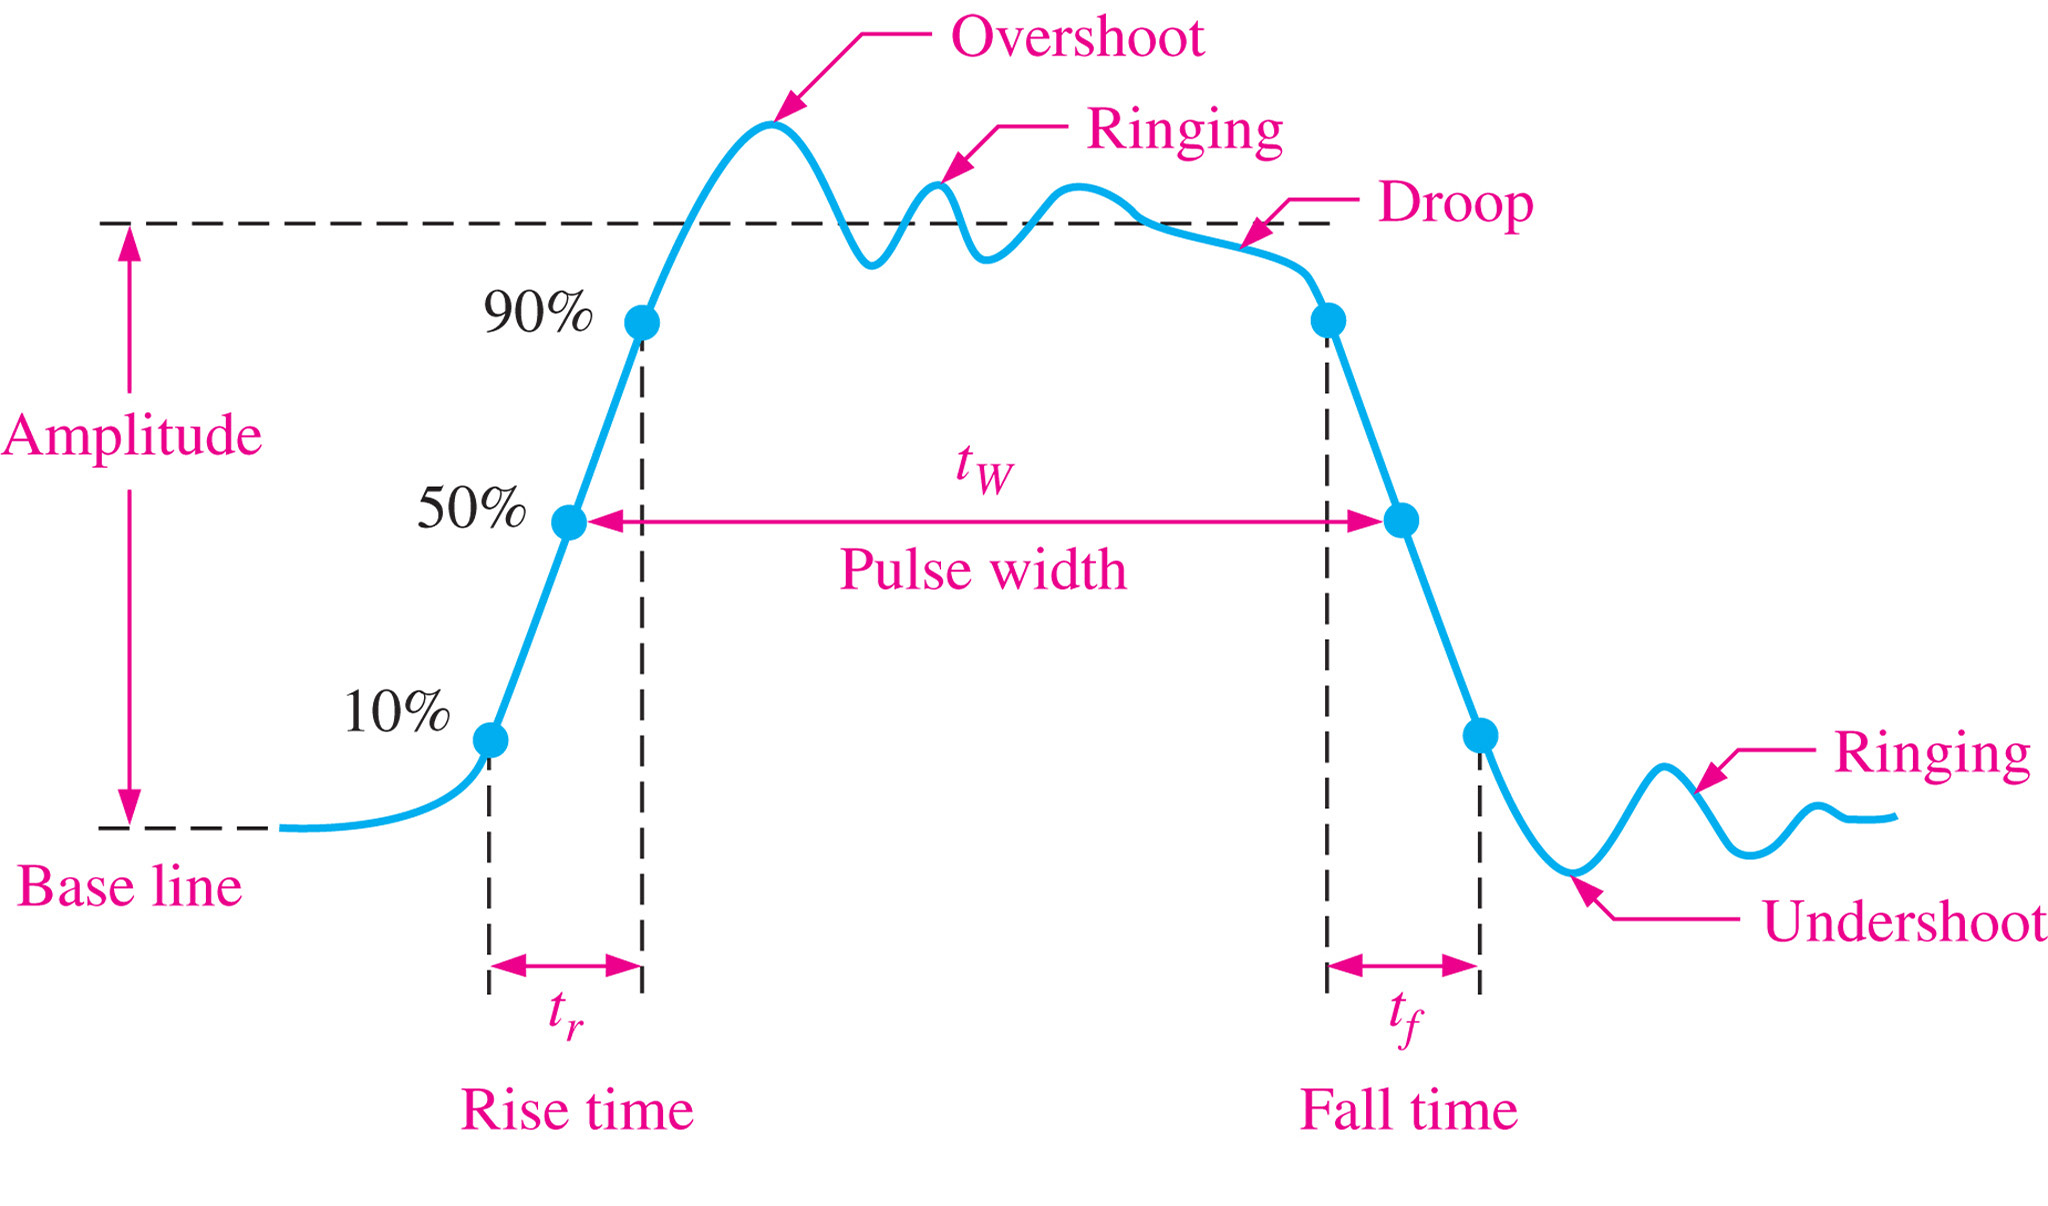
\includegraphics[width=0.4\textwidth]{figures/pulse2.jpg} \hspace{1cm}
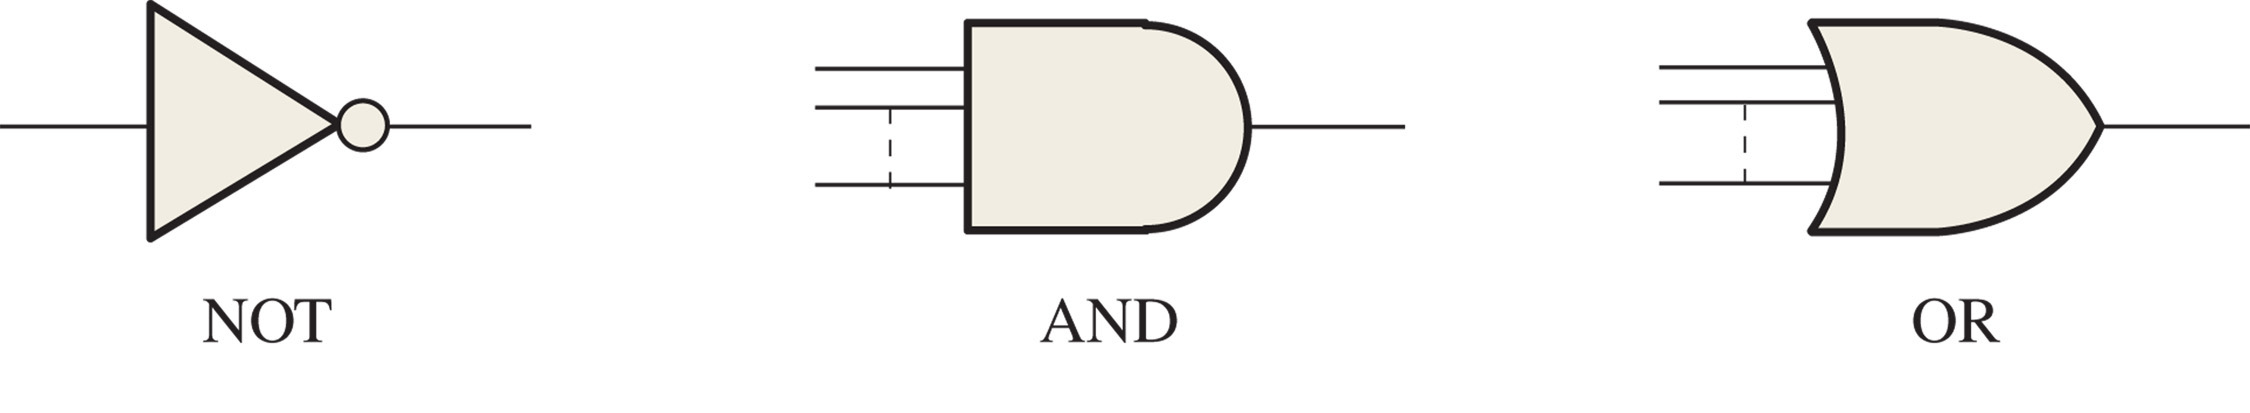
\includegraphics[width=0.4\textwidth]{figures/gate_0.jpg}
\caption{\label{fig:p} (Left) Properties of a digital pulse. (Right) Three basic logic gates.}
\end{figure}

\begin{enumerate}
\item A canonical digital pulse is depicted in Fig. \ref{fig:p} (left).  Digital components like logic gates have finite capacitance and input impedance that depends on frequency.
\begin{itemize}
\item Suppose the amplitude is CMOS HIGH (between 3.5V and 5V), and has a measured value of 3.55 V.  What are the 10\% and 90\% amplitudes? \\ \vspace{0.5cm}
\item Suppose we treat the rise as linear, and we label the time of the 10\% amplitude as $t=0$ $\mu$s.  If the rise occurs at 33 V/$\mu$s, when does the 90\% amplitude occur?  This is the rise time. \\ \vspace{0.5cm}
\item What is the pulse width, if the pulse width is 5 times the rise time? \\ \vspace{0.5cm}
\item If the next pulse always occurs two pulse widths from the initial rise, what are the period and frequency of the signal? \\ \vspace{0.5cm}
\end{itemize}
\end{enumerate}

\section{Logic Operations}

\begin{enumerate}
\item Three basic logic gates are depicted in Fig. \ref{fig:p} (right).
\begin{itemize}
\item What is the output bit stream from left gate if the input is: 1000 1000? \\ \vspace{0.25cm}
\item What is the output bit stream from the middle gate if the two input bit streams are: 1000 1000 and 1001 1001? \\ \vspace{0.25cm}
\item What is the output bit stream from the right gate if the two input bit streams are: 1000 1000 and 1001 1001? \\ \vspace{0.25cm}
\end{itemize}
\end{enumerate}

\end{document}
